\documentclass[tikz]{standalone}


\usepackage{graphicx}
\usepackage{pxfonts}
\newcommand{\figf}{\bfseries\sffamily}


\begin{document}

\sffamily



\begin{tikzpicture}[anchor = north west]

	\clip (0,0) rectangle +(18,-6.8);

	\begin{scope}[yshift=+2mm]
		\clip (0,0) rectangle +(7.8,-2.95);
		\node at (0,0) {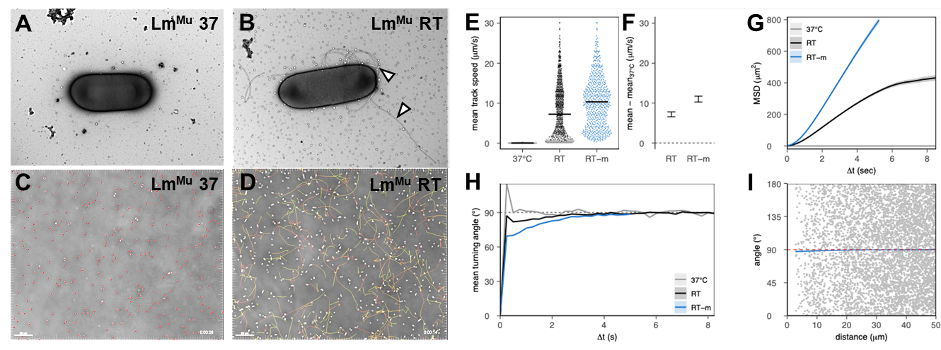
\includegraphics[page=1]{../img/figure1.png}};
		%\node at (0,0) {\figf A};
	\end{scope}
	
	\begin{scope}[yshift=-3mm]
		\clip (0,-3) rectangle +(7.8,-3);
		\node at (0,0) {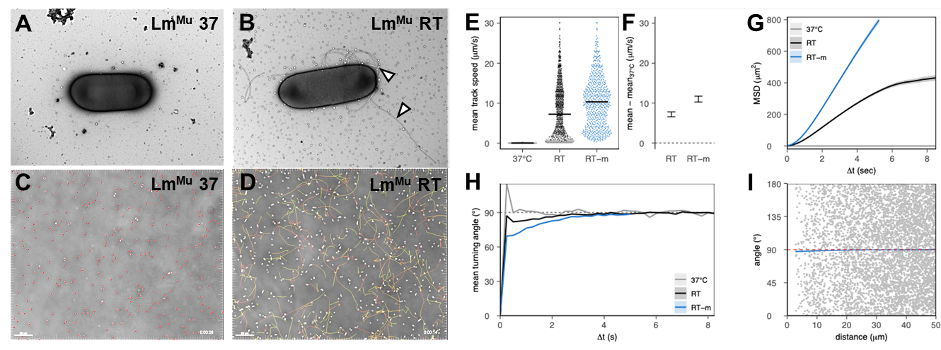
\includegraphics[page=1]{../img/figure1.png}};
		%\node at (0,0) {\figf A};
	\end{scope}

	\begin{scope}[xshift=8cm]
	 \node[scale=1] at (0,-0.3) {\includegraphics[page=1]{../plots/panelsE-I.pdf}};
	 \node at (0,-0.05) {\figf E};
	 \node at (4,-0.05) {\figf F};
	 \node at (5.8,-0.05) {\figf G};
	 \node at (0,-3.25) {\figf H};
	 \node at (5.8,-3.25) {\figf I};
	\end{scope}

	

\end{tikzpicture}

\end{document}